\documentclass[10pt]{article}

\usepackage{amsmath}% http://ctan.org/pkg/amsmath
\usepackage{amsthm}
\usepackage{todonotes}
\usepackage[margin=1in]{geometry}
\usepackage{algorithm}
\usepackage{url}
\usepackage[noend]{algpseudocode}
\usepackage{mdframed}
\usepackage{tikz}
\usepackage{enumerate}
\usetikzlibrary{matrix,shapes,arrows,positioning,chains, calc}

%% defining new theorem environment for definition
\newtheorem{defn}{\textbf{Definition}}
\newtheorem{thm}{\textbf{Theorem}}
\newtheorem{cor}{\textbf{Corollary}}
\newtheorem{lemma}{\textbf{Lemma}}

\renewcommand{\algorithmicrequire}{\textbf{Input:}}
\renewcommand{\algorithmicensure}{\textbf{Output:}}

\begin{document}
\title{IP/NDN Application-Layer Gateway Middleware}
\author{Christopher A. Wood \\ {\tt woodc1@uci.edu}}
\date{\today}
%\thanks{TODO}
\maketitle

%%%%%%%%%%%%%%%%%%%%%
%%% MAIN CONTENT
%%%%%%%%%%%%%%%%%%%%%

\section{Introduction}
At its core, the design and architecture of today's Internet is a communication-based packet switching network. Since its inception, it has been retrofitted with a variety of transport and application layer protocols and middleware to support a growing set of consumer applications, such as the Web, email, and perhaps most importantly in recent times, media streaming services. The latter type are bandwidth-intensive content distribution applications which leverage the underlying communication-based network as a distribution network, leading to a massive consumption of vital networking resources. 

Information-centric networks (ICNs) are a new class of network architecture designs that aim to address this increasingly popular type of network traffic by decoupling data from its source and shifting the emphasis from hosts and interfaces to content \cite{first}. By directly addressing content instead of hosts, content dissemination and security can be ``distributed'' throughout the network in the sense that consumers requests for content are satisfied by \emph{any} resource in the network (i.e., not necessarily the original producer). For example, routers close to consumers may cache content with a particular name and then satisfy all content requests that match the content's name. Inter-network caching and data-centric security measures are two of the defining characteristics of ICN designs. 

As of today there are several ICN proposals being explored as alternative designs to today's Internet; of all such projects, Named Data Networking (NDN) \cite{NDNtech} is one of the more promising designs that is still begin actively developed by universities, research labs, and companies worldwide (see \url{www.named-data.net} for more information). As a replacement for IP-based networks, the complete adoption of NDN, or any one of these designs, will realistically need to be done by slow and continual integration and replacement of IP-based networking resources with NDN-based resources. Currently, however, there is no engineering plan to support the IP-to-ICN interoperability during this integration. 

Consequently, the primary objective of this project is to aid the integration of future content-centric networking resources into the existing IP-centric Internet by providing an application-layer gateway between IP and NDN resources. Application-layer traffic corresponding to protocols such as HTTP, FTP, SMTP, IMAP, etc. will be translated by middleware running in such gateways to correctly interface with the NDN resources, thereby serving as a semantic bridge between these two fundamentally different networking architectures so that they may transparently coexist. 

\section{Overview}
The NDN architecture enables relevant content to be pushed and stored throughout the network to minimize overall bandwidth consumption. Network caches and addressable content, rather than addressable hosts or interfaces, promote reduced network congestion and latency by keeping content closer to its intended recipients. The process by which content is requested is through the issuance of an \emph{interest} - a unique and meaningful name for a piece of content. Interests are forwarded upstream towards the original producer using information in a \emph{forwarding interest base} (a routing table), which is populated using standard routing protocols. Routers that have cached content matching the interest name along the consumer-to-producer path, or producers who advertise that they provide content matching the name, may respond with the corresponding (cryptographically signed) piece of content. As a result, network flow is preserved since content traverses the same network path from which the interest originated. 

This content-based strategy for information retrieval is fundamentally different from IP-based content distribution. Therefore, in order to support the interoperability of applications across IP and NDN networks, the semantics of IP-based messages and NDN-based messages must be supported by some proxy. The proposed NDN gateway is intended to satisfy this role as a server and middleware software stack designed to support the translation between IP-based and NDN-based communication and messages. For example, HTTP GET requests would be intercepted and translated into an interest for the same piece of content. The procedure for such a translation consists of an IP-to-NDN resolution transformation (similar to a DNS query), message creation and transmission (e.g., HTTP GET to NDN interest), and response transformation (e.g., NDN content response to HTTP response). For application-layer protocols that maintain transport-layer state (e.g., persistent HTTP connections), TCP connection management will be automatically maintained at the gateway. This flow of messages is illustrated in Figure 1. 

\begin{figure}
\begin{center}
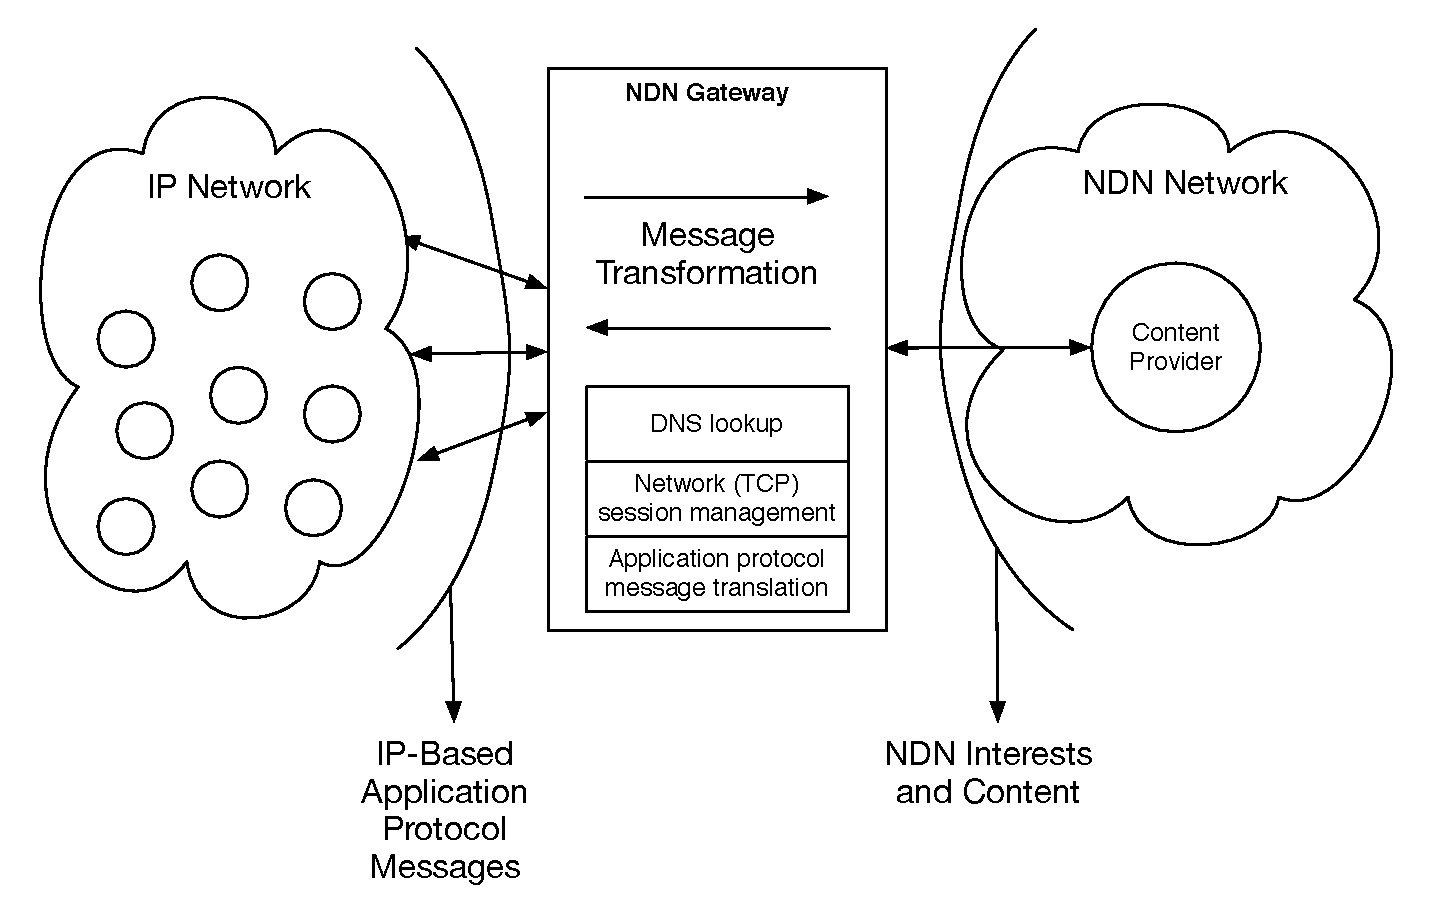
\includegraphics[scale=0.5]{../../sketches/gateway_highlevel.pdf}
\caption{System context diagram for the IP-to-NDN gateway.}
\end{center}
\end{figure}

\section{Implementation Highlights and Milestones}
The implementation of this project will be done using both C/C++ and Python and will rely on the open-source CCNx \cite{ccnx} library for all NDN-specific functionality. Architecturally, the middleware will be partitioned among a Python-based front-end for intercepting all IP-based traffic and performing application-layer protocol translation, a C-based backend utilizing the CCNx library to interface with NDN network resources, and, time permitting, a web interface that can be used to configure the gateway. Collectively, the deliverables for this project are a software design and architecture document, application gateway source code (Python and C/C++), performance metrics relevant to the operation and overhead of the gateway (e.g., message translation overhead, average message latency between applications traversing the gateway, etc), and a gateway configuration web interface. A preliminary timeline for the major milestones of this project is given below.

\begin{enumerate}[{\bf Week} 1:]
	\setcounter{enumi}{2}
	\item Project proposal and preliminary project experiments
	\item Front-end skeleton, API design, and application-layer protocol listeners
	\item Back-end skeleton, design, and NDNx integration
	\item Python IPC socket communication setup application-wide integration testing
	\item Middleware DNS lookup
	\item Middleware session management
	\item Middleware application layer translation and finalize project experiments
	\item Conduct experiments, gather performance measurements, and begin draft of final report 
	\item Finish report and (time permitting) develop elementary web interface for configuration
\end{enumerate}

%%%%%%%%%%%%%%%%%%%%%
%%% END MAIN CONTENT
%%%%%%%%%%%%%%%%%%%%%

%%% BIBLIOGRAPHY
\begin{thebibliography}{[MT1]}

\bibitem{first} V. Jacobson, D. K. Smetters, J. D. Thornton, M. F. Plass, N. H. Briggs, R. L. Braynard (PARC) Networking Named Content, CoNEXT 2009, Rome, December, 2009.

\bibitem{NDNtech} L. Zhang, D. Estrin, J. Burke, V. Jacobson, J. D. Thornton, D. K. Smetters, B. Zhang, G. Tsudik, K.C. Claffy, D. Krioukov, D. Massey, C. Papadopoulos, T. Abdelzaher, L. Wang, P. Crowley, and E. Yeh. Named Data Networking (NDN) Project. PARC Tech Report 2010-003, NDN-0001 (2010).

\bibitem{ccnx} Content Centric Networking (CCNx) - Project CCNx. Available online at: \url{https://github.com/ProjectCCNx/ccnx}. Last accessed: 4/2/14.

\end{thebibliography}

\end{document}
